\documentclass[letterpaper,12pt,fleqn]{article}
\usepackage{matharticle}
\usepackage{siunitx}
\pagestyle{plain}
\begin{document}

\begin{center}
\Large Math-1003b Homework \#11 Solutions
\end{center}

\vspace{0.5in}

\underline{Reading}

\bigskip

\begin{itemize}
\item Section 10.1
\end{itemize}

\bigskip

\underline{Problems}

\bigskip

\begin{enumerate}
\item Simplify:
  \[\sqrt[3]{\frac{64x^3y^6}{z^{12}}}=\sqrt[3]{\frac{4^3x^3(y^2)^3}{(z^4)^3}}
  =\sqrt[3]{\left(\frac{4xy^2}{z^4}\right)^3}=\frac{4xy^2}{z^4}\]

\item Simplify:
  \[\sqrt[4]{\frac{16x^4y^8}{z^{12}}}=\sqrt[4]{\frac{2^4x^4(y^2)^4}{(z^3)^4}}=
  \sqrt[4]{\left(\frac{2xy^2}{z^3}\right)^4}=\frac{2\abs{x}y^2}{\abs{z}^3}\]

\item You are standing 10 feet away from a 25 foot flagpole. How far away are you from
  the flag at the top of the pole?

  \begin{minipage}{2in}
    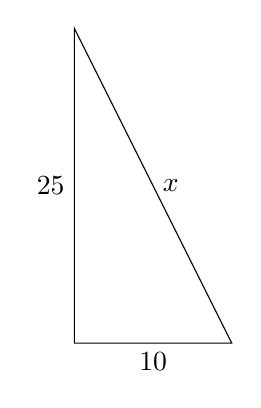
\begin{tikzpicture}
      \draw (0,0) -- node [below] {$10$} (2,0)
      -- node [right] {$x$} (0,4)
      -- node [left] {$25$} cycle;
    \end{tikzpicture}
  \end{minipage}
  \begin{minipage}{3in}
    $x^2=10^2+25^2$

    $x^2=100+625$

    $x^2=725$

    $x=\sqrt{725}=26.9$

    $\SI{26.9}{feet}$
  \end{minipage}

\item Find the domain:
  \begin{enumerate}
  \item $f(x)=\sqrt[4]{\frac{x+1}{x-2}}$

    This is an even root so that radicand cannot be negative:

    $\frac{x+1}{x-2}\ge0$

    \bigskip

    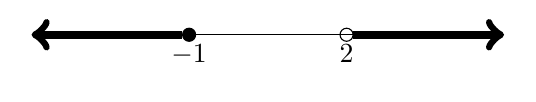
\begin{tikzpicture}
      \draw (-3,0) -- (3,0);
      \node [draw,circle,fill,scale=0.5] (a) at (-1,0) {};
      \node [draw,circle,scale=0.5] (b) at (1,0) {};
      \node [below] at (a) {$-1$};
      \node [below] at (b) {$2$};
      \draw [<-,line width=1mm] (-3,0) to (a);
      \draw [->,line width=1mm] (b) to (3,0);
    \end{tikzpicture}

    \bigskip

    $x\in(-\infty,-1]\cup(2,\infty)$

  \item $f(x)=\sqrt[3]{\frac{x+1}{x-2}}$

    This is an odd root so we don't need to worry about the radicand being negative;
    however, we do still worry about the pole at $x=2$:

    $x\in(-\infty,2)\cup(2,\infty)$
  \end{enumerate}
\end{enumerate}

\end{document}
